\begin{figure}[ht]
  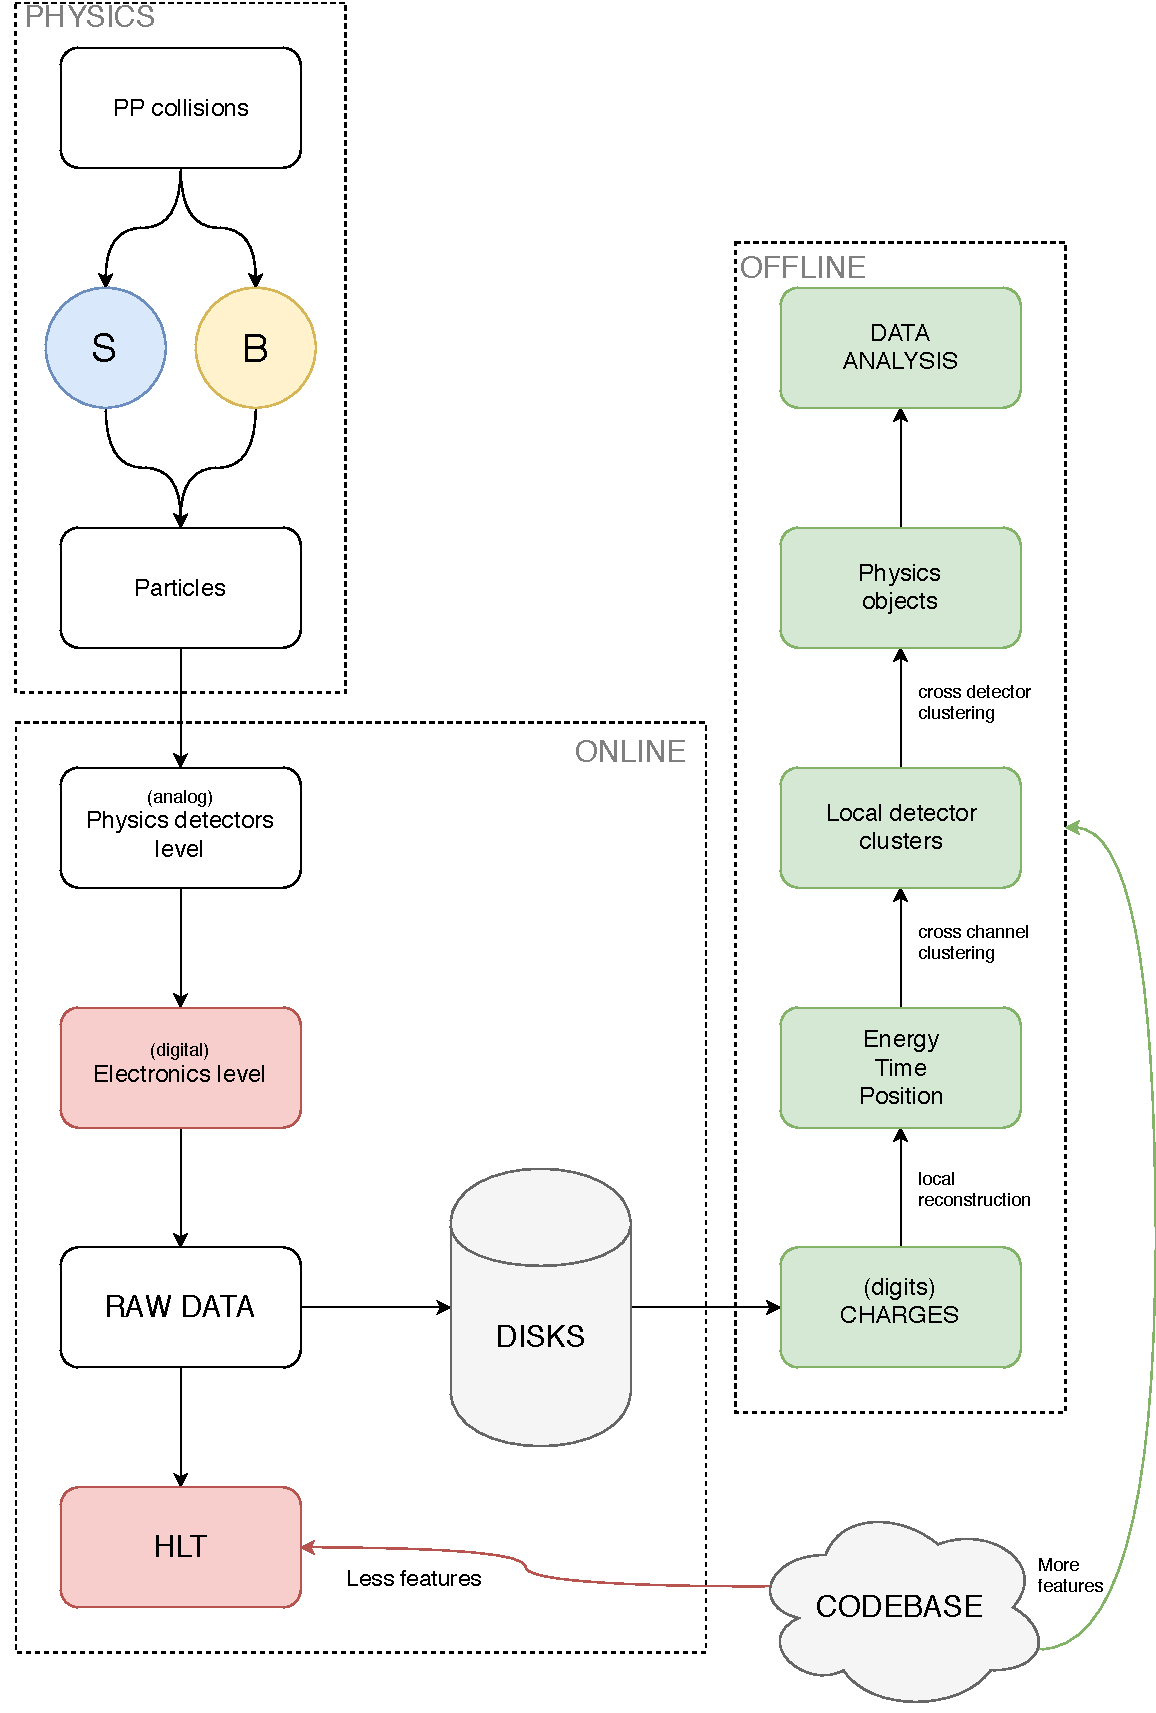
\includegraphics[height=\textheight]{img/dataflow}
  \caption{Cern data flow from collisions to analysis}
  \label{img:dataflow}
\end{figure}
% This might be an introduction
Modern high energy physics (HEP) requires analysis. To make it possible several large scale objects are needed: from accelerators, detectors, data centers to the thousands of people involved to design and run the infrastructure. Here at CERN everything starts with physics by colliding particles and everything ends with the physics performed by analyzing the data acquired. But, to produce the necessary data, in the right amount, a long and complicated process, showed in figure \ref{img:dataflow}, is involved. It is worth to briefly describe it to understand the reason of our work and where is it place inside it. \\
\paragraph{Data generation}
The process starts with \textbf{particle collisions} this lead to particle interactions that create some \textbf{intermediate product}. This intermediate product can not be directly observed, bit it decays in \textbf{particles} that go through the detectors. 
\paragraph{Data aquisition}
Detectors are split in two levels: \textbf{physics detector level} and \textbf{electronics level}. The physics level takes in input sensor readouts and produces an analog signal. This analog signal is the digitalized by the electronics level. This level also decides if the event is interesting or not, based on this the event is discarded or recorded. 
% Should I say that not interesting reading are discarded here?
The event that survive this ends up dumped into \textbf{disks} and send to the \textbf{High level trigger}. \\
It is important to notice that these decision are taken in real time, to meet the throughput and timing requirements everything is built with \textbf{asic}s and \textbf{fpga}s boards. 
\paragraph{Data processing}